\documentclass[12pt,a4paper]{article}
\usepackage[left= 3cm, right= 3.00cm, width=17.00cm, height=24.00cm]{geometry}
\usepackage[latin1]{inputenc}
\usepackage{amsmath}
\usepackage{amsfonts}
\usepackage{amssymb}
\usepackage{graphicx}
\usepackage{float}
\usepackage{subfigure}
\usepackage{placeins}
\usepackage{mathrsfs}
\usepackage{dirtytalk}
%\usepackage[T1]{fontenc}
%\usepackage[french]{babel}
%\usepackage[utf8]{inputenc}
%\usepackage{ytab}
%\usepackage{simplewick}
\begin{document}
\section{Packages Used}
\begin{itemize}
\item CountVectorizer Package: To convert a collection of document text into a matrix of token (i.e. word) counts. 
\end{itemize}

\begin{itemize}
\item TfidfVectorizer Package: To convert the words in a document into tf-idf (Term Frequency-Inverse Document Frequency) scores, which is a score for the relative importance of the words in the documents (corpus). First one computes the Term Frequency (TF):
\begin{align}
tf_{i,j}=\frac{n_{i,j}}{\sum_k n_{i,j}}
\end{align}
\noindent which is the number of times a word appears in a word document divided by the total number of words in the document. Then the Inverse Data Frequency (IDF) is computed next:
\begin{align}
idf(w)=\log\bigg(\frac{N}{df_t}\bigg)
\end{align}
which is the log of the number of documents divided by the number of documents that contain the word $w$. Then finally the TF-IDF is the multiplication of Tf and IDF:
\begin{align}
w_{i,j}=tf_{i,j}\times \log\bigg(\frac{N}{df_i}\bigg)
\end{align}
where $w_{i,j}$ is a word in a document.
\end{itemize}

\begin{itemize}
\item RandomOverSample package: The package is used for random over sampling for the minority classes/labels, which will increase the number of minority classes.
\end{itemize}

\section{Architect of the model}
\noindent The LinearSVC (Support Vector Classifier) it is a Support Vector Classifier model with a linear kernel. The model belongs to a family of SVM's (Support Vector Machines), the model fits the data by creating a best-fit hyperplane that divides or categorizes data. The dimensions of the hyperplane depends on the number of features, if the number of input features is 2, then the hyperplane will be a line (1 dimension), if the number of input features is 3, then the hyperplane will be 2-dimensional plane. See figure \ref{fig:svm} for better depiction of an SVC in two dimension.

\begin{figure}[h!]
\label{fig:svm}
\centering
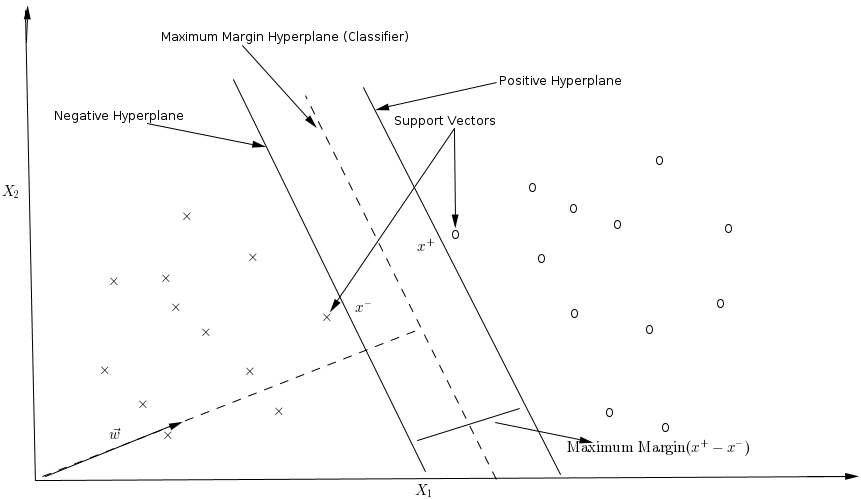
\includegraphics[scale=0.55]{svm_1}
\caption{Support Vector Classifier}
\centering
\end{figure}

\noindent  The vector points closest to the +ve and -ve hyperplanes are known as the support vectors, because it is only these two points contributing to the results of the classifier, and the other points are not necessarily contributing. Deleting the support vectors  will change the position of the hyperplane, whilst deleting data points that not support vectors will not change the position of the hyperplane. \\
\\
The distance of the support vectors from the maximum margin hyperplane is called the margin. The objective of the SVC model is to find a maximal margin that separates the two regions of data points from above. Mathematically the equation of a hyperplane is,
\begin{align}
y-ax-b=0,
\end{align}
and the dot product between two vectors $\vec{w}$ and $\vec{x}$:
\begin{align}
\vec{w} =\begin{bmatrix}
-b\\-a\\1
\end{bmatrix}\quad \vec{x}=\begin{bmatrix}
1\\x\\y
\end{bmatrix}
\end{align}

\noindent yields 
\begin{align}
\vec{w}^T\vec{x}=-b-ax+y
\end{align}

\noindent In Support Vector Classifiers we are looking for the condition,
\begin{align}
\vec{w}^T\vec{x}+b=0
\end{align}

\noindent where $w$ can be described as a weight of the model and $b$ as the bias term. Also the weight vector will be perpendicular to the Maximum hyperplane as shown in figure \ref{fig:svm}.  As illustrated in the figure above, to find the maximum margin we take the dot product of the difference between the support vectors $x^+$ and $x^-$ with the normilised weight vector $w$:
\begin{align}
(x^+-x^-)\cdot \frac{w}{|w|}=x^+\cdot\frac{w}{|w|}-x^-\cdot\frac{w}{|w|}.
\end{align}

\noindent Maximising the margin is equivalent to minimizing the loss function which is the hinge function,
\begin{align}
L(w)=\sum_{i=1}\underbrace{max(0,1-y_i[\vec{w}^T\vec{x}+b])}_{Loss function}+\underbrace{\lambda|\vec{w}|^2}_{regularization}
\end{align}

\noindent where $\lambda$ is equal to $\frac{1}{C}$ parameter. The purpose of the first term (loss function) in the hinge function is to penalize the model for misclassifications, it measures the error due to misclassifications. The function of the second term (regularization parameter) in the hinge loss is to avoid overfitting the model by penalizing it for large coefficients in the solution vector, and the regularization coefficient $\lambda$  determines the trade-off between increasing the margin size and making sure the input data $x$ is placed in the correct side of the margin.\\
\\
\noindent The kernel functions in SVC and SVM's help to transform data from low dimension into higher dimension for easier classification. For example, consider below, a linear data in 1-dimensional space where the data is defined by the function $f(x)=x$, it is difficult to draw a line (hyperplane) in order to separate and classify the  data,


\begin{figure}[h!]
\label{fig:svm}
\centering
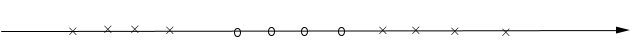
\includegraphics[scale=0.55]{svm_2}
\caption{1 dimensional data defined by $f(x)=x$}
\centering
\end{figure}

\noindent However this data can be transformed into a 2-dimensional space and be defined by the function $f(x)=x^2$ as shown below,

\begin{figure}[h!]
\label{fig:svm}
\centering
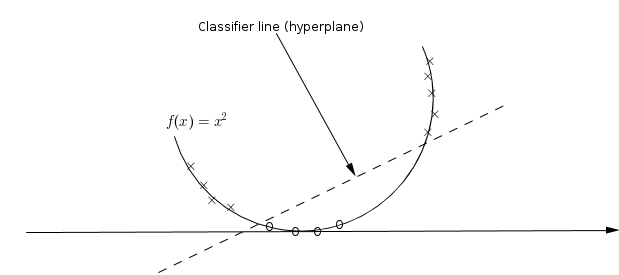
\includegraphics[scale=0.55]{svm_3}
\caption{1 dimensional data defined by $f(x)=x^2$}
\centering
\end{figure}

\noindent Now it is easier to draw a line (hyperplane) and classify the data.

\section{Procedure and Results}

Since there was class imbalance in the data, random over sampling was performed, in order to increase the number of minority classes. After doing random sampling the data was pre-processed, by removing commas and converting all the words into lowercases, it was not a good idea to remove stop words since they are important for language classification.\\
\\
\noindent The data was split into train and test data, and the LinearSVC model was trained on 30 percent of the data, and tested on 70 percent of the data. The accuracy of the model on tested data was found to be 97.45 percent and the precision, recall and f1 scores where all above 90 percent for all the three classes, which shows the model doesn't have a bias prediction on any class.


\section{Bonus Questions}

1.  Alternative models that can be used to solve the tasks are Recurrent Neural Networks (RNN) and Random Forest classifier. For the recurent neural networks we will need to use word embeddings to convert the text data into numerical data then the model will be trained by storing both the words in a document and the the documents inside the hidden states (memory) of the model, these hidden states will function as a memory of the model, these memories will assist the model to make correct prediction, since words and documents related to different languages will be stored in different memories (hidden) states.  \\
\\
The Random Forest will build a decision tree. Each node model will split the dataset into two nodes, using a randomly selected feature that optimizes the split quality using the Gini criteria. The model will create a multiple number of individual trees that will operate as an ensemble. Then each tree will have an opportuninty to make a class/label prediction, then a class with the most vote will become the model's overall prediction.\\
\\
2. Supervised learning involves training a model with data that has labels or classes, the labels helps to direct the gradients of the weights toward an optimum.\\
\\
\noindent In unsupervised learning the model is trained without any labeled data. The model has to discover patterns and hidden structures from the data without any assistance.\\
\\
3. Classification has to do with labels that are discrete, it is about training a model with labeled data in order for the model to predict labels. Regression has to do with continous values or quantity, the model is trained with an output data that is continous, the model is trained to predict continous values or quantities.\\
\\
4.Data with class imbalance will lead into the model being biased towards the prevalent class, the accuracy of the model can also be misleadingly high, since the model might only predict the prevalent class.\\
\\
5. To mitigate class imbalance we can use a random over sampling technique where the number of the under represented (minority) class is replicated several times so that they are fairly represented. We can also do the opposite and use random under sampling technique where the number of majority class is randomly reduced or removed from the the data.\\
\\
6. Deep learning has to do with artificial neural networks (ANN), deep learning models are models that are built using ANN structures. Non-deep learning methods could be machine learning methods that are built without ANN structures. These methods might have  to do with models that learn from the data, then they apply what they have learned from the data. This may include both classical supervised and unsupervised models such as SVM, KNN and Kmeans clustering models. 





\end{document}